\documentclass[12pt,a4paper]{article}\usepackage{graphicx, color}
%% maxwidth is the original width if it is less than linewidth
%% otherwise use linewidth (to make sure the graphics do not exceed the margin)
\makeatletter
\def\maxwidth{ %
  \ifdim\Gin@nat@width>\linewidth
    \linewidth
  \else
    \Gin@nat@width
  \fi
}
\makeatother

\definecolor{fgcolor}{rgb}{0.2, 0.2, 0.2}
\newcommand{\hlnumber}[1]{\textcolor[rgb]{0,0,0}{#1}}%
\newcommand{\hlfunctioncall}[1]{\textcolor[rgb]{0.501960784313725,0,0.329411764705882}{\textbf{#1}}}%
\newcommand{\hlstring}[1]{\textcolor[rgb]{0.6,0.6,1}{#1}}%
\newcommand{\hlkeyword}[1]{\textcolor[rgb]{0,0,0}{\textbf{#1}}}%
\newcommand{\hlargument}[1]{\textcolor[rgb]{0.690196078431373,0.250980392156863,0.0196078431372549}{#1}}%
\newcommand{\hlcomment}[1]{\textcolor[rgb]{0.180392156862745,0.6,0.341176470588235}{#1}}%
\newcommand{\hlroxygencomment}[1]{\textcolor[rgb]{0.43921568627451,0.47843137254902,0.701960784313725}{#1}}%
\newcommand{\hlformalargs}[1]{\textcolor[rgb]{0.690196078431373,0.250980392156863,0.0196078431372549}{#1}}%
\newcommand{\hleqformalargs}[1]{\textcolor[rgb]{0.690196078431373,0.250980392156863,0.0196078431372549}{#1}}%
\newcommand{\hlassignement}[1]{\textcolor[rgb]{0,0,0}{\textbf{#1}}}%
\newcommand{\hlpackage}[1]{\textcolor[rgb]{0.588235294117647,0.709803921568627,0.145098039215686}{#1}}%
\newcommand{\hlslot}[1]{\textit{#1}}%
\newcommand{\hlsymbol}[1]{\textcolor[rgb]{0,0,0}{#1}}%
\newcommand{\hlprompt}[1]{\textcolor[rgb]{0.2,0.2,0.2}{#1}}%

\usepackage{framed}
\makeatletter
\newenvironment{kframe}{%
 \def\at@end@of@kframe{}%
 \ifinner\ifhmode%
  \def\at@end@of@kframe{\end{minipage}}%
  \begin{minipage}{\columnwidth}%
 \fi\fi%
 \def\FrameCommand##1{\hskip\@totalleftmargin \hskip-\fboxsep
 \colorbox{shadecolor}{##1}\hskip-\fboxsep
     % There is no \\@totalrightmargin, so:
     \hskip-\linewidth \hskip-\@totalleftmargin \hskip\columnwidth}%
 \MakeFramed {\advance\hsize-\width
   \@totalleftmargin\z@ \linewidth\hsize
   \@setminipage}}%
 {\par\unskip\endMakeFramed%
 \at@end@of@kframe}
\makeatother

\definecolor{shadecolor}{rgb}{.97, .97, .97}
\definecolor{messagecolor}{rgb}{0, 0, 0}
\definecolor{warningcolor}{rgb}{1, 0, 1}
\definecolor{errorcolor}{rgb}{1, 0, 0}
\newenvironment{knitrout}{}{} % an empty environment to be redefined in TeX

\usepackage{alltt}
%%%%%%%%%%%%%%%%%%%%导言区%%%%%%%%%%%%%%%%%%%%%%%%
\usepackage{fontspec}
\usepackage{xeCJK}
\usepackage{bbding} %使用特殊图下图像标志
\usepackage{graphicx} %插入图片
\usepackage{hyperref} %为了生成超链接
\usepackage{amsmath}
\setmainfont{Times New Roman}%缺省英文字体 Times New Roman                          
\setCJKmainfont{楷体_GB2312}%衬线字体 缺省中文字体为    

%%%%%%%%%%%%%%%%%%%%%%%%%%%%%%%%%%%%%%%%%%%%

%%%%%%%%%%%%%%%%%%%自定义命令%%%%%%%%%%%%%
%\renewcommand{item}[1]{\textbf{1}}

%%%%%%%%%%%%%%%%%%%%%%%%%%%%%%%%%%%%%%%%%%

\title{一份(不那么)简短的S4类的介绍\\[2ex]R中的面向对象的编程}
\author{Christophe Genolini著{ }\\ HatMatrix翻译}
\IfFileExists{upquote.sty}{\usepackage{upquote}}{}

\begin{document}




\maketitle
\tableofcontents

\part{初步}
\section{介绍}
这是一份对于R(或者S4类)的面向对象编程的指导。它不需要事先了解面向对象编程的,但是少量的关于R
的知识和对编程的大致了解还是必须的。对于那些完全的新手来说,看看章节D和第66提供的一些手册和书籍。
\subsection{序言:哲学和计算机科学}
你将要阅读一本关于面向对象编程的指导手册,你将因此学习一种新的方法。你将或知道不是存在“一种”而是“很多种”编程的方法:在这个议题上,数据处理专家并不总是同意。
这份指导手册紧跟当前的观点(XXX)。一些非常有能力的人同意这一点,另外一些这不同意……所以这份手册讲过出现好几种观点。
因此,警告读者,在你手中握有所有的元素,你又能力自己来判断并且自由地选择你自己的概念,知识之光……它是没有生命的盛大?(法语的Elle n’est pas
belle la vie?Google翻译的,不知道什么意思)

\subsection{什么是S4}
S4是S语言的第四版本。S语言有两种实现:商业的S-plus和自由的R。s4向比较与S3增加的主要特性是开发函数的时候允许把S语言当作是一门面向对象的语言\footnote{允许当作面向对象的不知转换为面向对象的,在任何情况下,R都不是一门面向对象的语言,仍然是一门传统的编程语言,使用进一步的封装来解释(XXX),迫不及待想发现R++了(类比c和c++——译注)}。通过扩展,S4代表了S语言的面向对象编程,因此也代表了R和S-plus的面向对象的编程。

\subsection{什么是面向对象的编程}
一个对象是一些列变量和函数的集合,他们关注的是同一个主题——这个对象本身。是不是很不清晰?让我们来据一个例子:一个称之为“image”的对象包含了多个变量,这些变量(比如像图像的大小,压缩的模式,图像本省)使得定义图像变得可能并且包含一些用于处理这个图像的函数(比如blackAnWhite()函数或者resizing()函数)。

\subsection{为什么要使用面向对象编程}
作为一个新手来说,面向对象是一个复杂的东西并且其优势并补那么明显:它必须在事先考虑好程序的各个方面,对问题的建模,对类型的选择,对包含其中的各个对象之间的联系等等都要有考虑。各种缺点。因此,很合理的一个问题是:为什么要使用面向对象编程呢?
\subsubsection{传统编程}
让我们据一个例子来比较传统的编程和面向对象编程的区别。BMI(Body Mass Index,体重指数)是一个衡量胖瘦的度量,是通过体重(千克)除以身高(米,原文说的是厘米,应该有误)的平方。那么,可以得出:
\begin{itemize}
  \item 20<BMI<25:一切安好
  \item 25<BMI<30:泰迪熊
  \item 30<BMI<40:柔软舒适的泰迪熊
  \item 40<BMI:大泰迪熊,具有双倍的柔软度,但是应该尽快去看医生了
  \item 18<BMI<20:芭比娃娃
  \item 16<BMI<18:芭比娃娃模特
  \item BMI<16:芭比骷髅,和大泰迪熊一起去看医生吧,注意了哦
\end{itemize}
所以我们想计算BMI值,在传统编程中,再简单不过了:
\begin{knitrout}
\definecolor{shadecolor}{rgb}{0.969, 0.969, 0.969}\color{fgcolor}\begin{kframe}
\begin{alltt}
\hlcomment{# 传统方法计算BMI}
weight <- 85
size <- 1.84
(BMI <- weight/size^2)
\end{alltt}
\begin{verbatim}
## [1] 25.11
\end{verbatim}
\end{kframe}
\end{knitrout}

到现在为止,没有什么神秘的。如果你想极端两个人——"Me"和"Her"的BMI,你将会这么做:
\begin{knitrout}
\definecolor{shadecolor}{rgb}{0.969, 0.969, 0.969}\color{fgcolor}\begin{kframe}
\begin{alltt}
\hlcomment{# 传统编程计算我的BMI}
weightMe <- 85
sizeMe <- 1.84
(BMIMe <- weightMe/sizeMe^2)
\end{alltt}
\begin{verbatim}
## [1] 25.11
\end{verbatim}
\begin{alltt}
\hlcomment{# 传统编程计算她的BMI}
weightHer <- 62
sizeHer <- 1.6
(BMIHer <- weightMe/sizeHer^2)
\end{alltt}
\begin{verbatim}
## [1] 33.2
\end{verbatim}
\end{kframe}
\end{knitrout}

可以工作的哦……只是"Her"被称之为“舒适的泰迪熊”,可是她的体重没有特别重啊!小小检查一下代码就会很快地发现一个小错误:在计算\textbf{BMIHer}的时候是错的,我们用\textbf{sizeHer}除以\textbf{weightMe}而不是\textbf{sizeHer}除以\textbf{weightHer}。自然地,R没有发现错误:从它的观点来看,它做的只是把两个数字相除而已。

\subsubsection{面向对象编程}
在对象语言中,方法是不同的。必须在定义了包含两个值———\textbf{weight}和\textbf{size}以后才能开始定义方法。然后,必须要定义一个\textbf{show}函数来展示BMI\footnote{为了构造的例子立即重现,我们需要定义一些对象。我们这样做没有解释为什么,但是是很自然的,这些在随后都会详细地解释}。
\begin{knitrout}
\definecolor{shadecolor}{rgb}{0.969, 0.969, 0.969}\color{fgcolor}\begin{kframe}
\begin{alltt}
\hlcomment{# 定义一个BMI对象}
\hlfunctioncall{setClass}(\hlstring{"BMI"}, \hlfunctioncall{representation}(weight = \hlstring{"numeric"}, 
    size = \hlstring{"numeric"}))
\hlfunctioncall{setMethod}(f = \hlstring{"show"}, signature = \hlstring{"BMI"}, definition = \hlfunctioncall{function}(object) \{
    \hlfunctioncall{cat}(\hlstring{"BMI="}, object@weight/(object@size^2), \hlstring{"\textbackslash{}n"})
\})
\end{alltt}
\begin{verbatim}
## [1] "show"
\end{verbatim}
\end{kframe}
\end{knitrout}

然后,这段代码等于在章节1.4.1的第3页中的那样:
\begin{knitrout}
\definecolor{shadecolor}{rgb}{0.969, 0.969, 0.969}\color{fgcolor}\begin{kframe}
\begin{alltt}
\hlcomment{# 为我建立一个对象,并且发布我的BMI}
(myBMI <- \hlfunctioncall{new}(Class = \hlstring{"BMI"}, weight = 85, size = 1.84))
\end{alltt}
\begin{verbatim}
## BMI= 25.11
\end{verbatim}
\begin{alltt}
\hlcomment{# 为她建立一个对象,并且发布她的BMI}
(herBMI <- \hlfunctioncall{new}(\hlstring{"BMI"}, weight = 62, size = 1.6))
\end{alltt}
\begin{verbatim}
## BMI= 24.22
\end{verbatim}
\end{kframe}
\end{knitrout}

当初始化是正确的时候(在传统编程中这也会出现问题的),不会又别的错误再发生。这依赖与对象的强大:程序的设计防止了某种类型的错误。
\begin{description}
  \item[类型:]对象可以防止类型错误。类型错误发生在必须使用某种类型的时候使用了另外一种类型。比如,把一个字符串加到了数字类型的变量上。这或多或少可以这么说——就是把一个苹果和一千米相加而不是把一个苹果和一个苹果相加。面向对象会阻止这么做:
\begin{knitrout}
\definecolor{shadecolor}{rgb}{0.969, 0.969, 0.969}\color{fgcolor}\begin{kframe}
\begin{alltt}
\hlcomment{# 传统编程,没有类型}
(weight <- \hlstring{"hello"})
\end{alltt}
\begin{verbatim}
## [1] "hello"
\end{verbatim}
\begin{alltt}
\hlcomment{# 面型对象编程}
\hlfunctioncall{new}(\hlstring{"BMI"}, weight = \hlstring{"Hello"}, size = 1.84)
\end{alltt}


{\ttfamily\noindent\bfseries\color{errorcolor}{\#\# Error: invalid class "BMI" object: invalid object for slot "weight" in class "BMI": got class "character", should be or extend class "numeric"}}\end{kframe}
\end{knitrout}


  \item[有效性检查:]对象能够使用“相关性检察员”来检查对象是不是符合一定的规则。比如,有的可能拒绝接受负的身高:
\begin{knitrout}
\definecolor{shadecolor}{rgb}{0.969, 0.969, 0.969}\color{fgcolor}\begin{kframe}
\begin{alltt}
\hlcomment{# 传统陪你和编程,没有限制}
(SizeMe <- -1.84)
\end{alltt}
\begin{verbatim}
## [1] -1.84
\end{verbatim}
\begin{alltt}
\hlfunctioncall{setValidity}(Class = \hlstring{"BMI"}, method = \hlfunctioncall{function}(object) \{
    \hlfunctioncall{if} (object@size < 0) \{
        \hlfunctioncall{return}(\hlstring{"negative Size"})
    \} else \{
        \hlfunctioncall{return}(TRUE)
    \}
\})
\end{alltt}
\begin{verbatim}
## Class "BMI" [in ".GlobalEnv"]
## 
## Slots:
##                       
## Name:   weight    size
## Class: numeric numeric
\end{verbatim}
\begin{alltt}
\hlfunctioncall{new}(\hlstring{"BMI"}, weight = 85, size = -1.84)
\end{alltt}


{\ttfamily\noindent\bfseries\color{errorcolor}{\#\# Error: invalid class "BMI" object: negative Size}}\end{kframe}
\end{knitrout}

  \item[继承:]面向对象的语允许像从其他的对象继承属性一样来定义对象,因此成为那个对象的儿子。这个子对象因此从其父对象那里获得所有存在的财富(指获得其所有的属性———译注)比如,打算对我们的诊断有一点点改进,我们加上了根据人的性别来进行判断。我们因此要定义新的对象——BMIplus,这个对象包括三个值:weight,zize和sex。前两个值和对象BMI中出现的是一样的。因此我们定义对象BMIplus的时候可以把其作为BMI的字对象,这样做可以让我们获得我们为BMI定义的函数show,而且我们没有做任何额外的工作,因为BMIplus继承了BMI。
\begin{knitrout}
\definecolor{shadecolor}{rgb}{0.969, 0.969, 0.969}\color{fgcolor}\begin{kframe}
\begin{alltt}
\hlcomment{# 继承的定义}
\hlfunctioncall{setClass}(\hlstring{"BMIplus"}, \hlfunctioncall{representation}(sex = \hlstring{"character"}), 
    contains = \hlstring{"BMI"})
he <- \hlfunctioncall{new}(\hlstring{"BMIplus"}, size = 1.76, weight = 84, sex = \hlstring{"Male"})
he
\end{alltt}
\begin{verbatim}
## BMI= 27.12
\end{verbatim}
\end{kframe}
\end{knitrout}

这种特性的威力将在章节4.2中更加清晰地显现。

  \item[封装:]最后,面向对象的语言允许我们定义所有关于对象的工具并且把他们锁起来,我们没有必要再打理会它们。这就叫作封装。汽车可以作为解释封装的一个很好的例子:一旦引擎盖关闭了,我们就不需要再知道机器行驶的任何细节。相同地,一旦对象完成了并且关闭了,那么用户就不再需要担心其工作程序。更好的是,我们考虑下汽车就会发现我们不可能犯错或者把汽油加到冷却箱中,因为冷却箱是无法接触到的。相同的方式,封装保护了那写必须被保护的,能够接触到的是那写没有风险的。
\end{description}

\subsection{总结}
面向对象编程”迫使“程序员有一个初步的反思。要很少有可能写处”快但是脏“的代码来,变成计划是必不可少的。特别是:
\begin{itemize}
  \item 对象必须声明和定义类型
  \item 控制机制能够检查对象内部的一致性
  \item 一个对象可以继承另外一个已经被定义的对象
  \item 最后,对象允许程序的封装:一但一个连接到程序的对象和函数被定义了,我们就不再需要处理对象内部的工具。
\end{itemize}

\subsection{程序的不为人知的一面}
完成了这个常常的介绍,插入一个题外话:当人们开始送火箭上太空\footnote{或者当人们把股票交易,医院,工资单等等的控制交给电脑的时候},在飞行中他们爆炸了,他们抹去伤心的眼泪寻求失败的原因。因为有人被烧死了,所以他们寻找责任人。他们找到了计算机科学专家。“声明下,这不是我们的错,这对计算机来说是一个既定的事实:所有的程序都存在错误!”不同的是这种情况下,出现错误的代价是相当高的。
所以,有经验的人和聪明的人开始思考寻找一种可以组织错误出现的编程方式。他们创建新的语言并且定义了新的编程规则。这被称之为整洁的编程或者称之为好的实践(你将会在59页的附录B节的发现看到一些好的行为的建议)。一些操作、做法、和编程的方法因此被称之为好的或者是整洁的,相反,另外的一些则被称之为坏的危险的甚至是肮脏的\footnote{这个由计算机科学专家贡献的术语的在法语中称之为crade,anythink like that igz English?}。这些评价的词汇中不含有道德的评价,这仅仅是在提及到编程错误的时候对编程方式的评价。因此坏的编程方式必须忽略。

\scalebox{4}{\HandRight}【个人观点】:R不是一门很纯净的语言。当一个程序员(或者是一个研究员)想要添加一个新的包的时候,它几乎可以自由地完成他想做的任何事情。这是非常棒的事情。但是他们总是可以自由地作出很多令人”惊讶“的事情\footnote{惊讶的是事情是指那些用户没有意料到的东西。比如,我们知道numberic()指的是一个空的数值型的对象,那么你期望一个空的matrix对象指的是什么呢?还有什么比matrix()更加令人“惊讶的”。R充满了惊喜(参看4.6节就能知道怎么表示一个空的matrix},这就显得有点弱了。所以R允许用户作出很多危险的操作。有时候通过禁止自身进行某些操作来使其更加清晰,但是情况并非总是如此,我们将会被带入去使用不适合的工具。但是我将使用本节开头的标识来指示危险的部分(我看来是危险的)。
\centerline{可能你从来没有被程序的不为人知的那一面坑过~} 

\section{概论}
一个对象是由围绕一个核心概念的一系列高度相关的函数和值组成的。正式说来,一个对象是由三个元素组成的:
\begin{itemize}
  \item 对象的名字,我们称之为\emph{类}。它也是整个对象的架构(由一个变量列表和函数组成)
  \item 对象的变量名,我们称之为\emph{槽}
  \item 对象的函数,我们称之为\emph{方法}
\end{itemize}
在介绍部分,我们已经定义了BMI类的对象。它的槽是weight和size,他的方法是show。
\subsection{槽}
槽是简单的被定义了类型的变量。一个被定义了类型的变量是一个其本质已经被固定了的变量。在R中,我们可以写weight <- 62(在这里,weight是个numberic模式的值),然后我们weighr <- "hello"(weight变成了character模式的值)。变量weight的类型是会变化的。
在面向对象编程中,是不怎么可能改变槽的类型的\footnote{很不幸的是,在R
和S4中,这是可能的。但是由于这是计算机科学史上毫无疑问的最肮脏的操作,我们最好“忘记”并且假装是不可以改变的。}这似乎是一种约束,但是事实上更加安全了。事实上,如果一个变量是用过weight来建立的,那么就完全没有理由能够接受到一串字符啊。

\subsubsection{方法}
我们区分4中可以运用到对象中的操作:
\begin{description}
  \item[建立方法:]这个类别包括所有用于建立对象的方法。最重要的一个称之为构造器。但是对于用户来说,它的使用有点粗糙。所以(友好的)程序员会写出容易接受的方法来创建对象(比如\textbf{numneric}来建立一个数值变量或者\textbf{read.csv}来创建一个数据框)。
  \item[验证:]在面向对象编程中,很有可能要检查槽是不是遵守某种规律。也很有可能根据计算其他属性来创建槽。所有的这些都是对象检验的一部分。
  \item[槽的处理:]修改和读取槽的值不像在传统编程中那么简单。因此,必须致力于钉地操作处理槽的方法(比如,names和names <- )。
  \item[其他:]对于每一个对象来说,先前说的都是一种“最低的要求”,还有很对对于对象来说特定的方法,特别是发布(posting)方法和计算(calculation)方法。
\end{description}
方法是又类型的对象。这种函数包含了两部分:\emph{input}和\emph{output}。输入的类型是函数的参数的类型的集合。输出值的类型是函数返回值的类型。函数的类型是outputType <- inputType。记做output <- function(inputType)。
比如,计算trace计算矩阵秩。因此它的类型是numeric <- trace(matrix)。

\subsubsection{画图就是胜利}
长篇大论不如一图了然。这句格言可以很好地运用于画图。没一个类使用一个矩形来表示,在矩形中指出它们的方法和槽,并且会指出它们的类型。两个类之间的继承关系(参看42页的9节)通过箭头来表示,从子对象只想父对象。
我们的对象BMI看起来就想下面这样。
\begin{figure}[htbp]
\centering
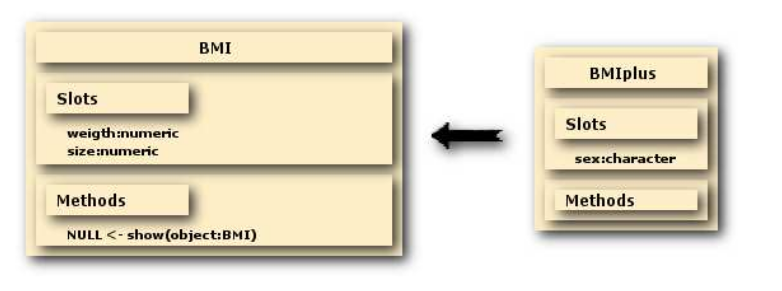
\includegraphics[width=5in]{./screenshot01.png}
\caption{}
\label{}
\end{figure} 

\section{例子}
不介绍像”wiz”,"spoun"或者是充满了数学方程的复杂的概念,这里介绍的是一个真实的例子:Tam医生的关于节食的工作。周复一周的,她在测量患者的BMI(比如说是17然后是17.2,然后是17.3)。对于一个病人来说,这一系列的观测序列就形成了一个trajectory(比如说,3周的观测值就是(17,17.2,17.3))。然后,Tam根据非常精确的标准来对她病人进行分类,这个标准是这样的[体重是不是增加了](是/不是)或者是[要求建他们的父母](是/不是/拒绝)或者是[很快又要进食](是/不是)。最后,Tam的目的是比较几种不同的分类方式的分类结果。
在这份指导手册中,我们会简化这个例子,仅仅保留我们用来介绍S4概念的那一部分。对于这个问题的完整的处理感兴趣的读者,有一个已经编写好的Kml包可以解决这个问题。这个包可以在CRAN和Kml的网站上获得。
\subsection{分析问题}
这个问题可以被分解为3个对象:
\begin{itemize}
  \item 第一对象包含病人的trajectories
  \item 第二个对象代表的是重新分配的组(我们称之为一个分配)
  \item 第三个对象是前两个的混合:把trajectories分配到组里面
\end{itemize}

\subsubsection{对象Trajectories}
Tam敬告我们说,对于一个给定的组,测量是每隔一周或者两周进行一次的。对象Trajectories必须考虑到这一点。这对对象是由两个槽来定义的:
\begin{description}
  \item[time:]表示的是每次测量进行的时间,为了简化,我们把这个跟踪调查的开始设为1。
  \item[traj:]表示的是病人BMI轨迹
\end{description}
举个例子:
\[time=(1,2,4,5)\]
\[traj=\begin{pmatrix}15 & 15.1 & 15.2 & 15.2\\
16 & 15.9 & 16 & 16.4\\
15.2 & 15.2 & 15.3 & 15.3\\
15.7 & 15.6 & 15.8 & 16
\end{pmatrix}\]
这个对象的方法是什么?Tam说在这种研究中,经常会有数据的缺失,所以知道缺失多少数据是很重要的,于是我们定义的第一个方法就是计算缺失值的个数。
第二个方法被放置在对电工Trajectories和对象Partition之间\footnote{在传统的面向对象编程语言中,每一个方法必须需与特定的类。在R中,这不是很重要的事情,因为一个方法不需要和一个类向关联。但是为了兼容传统的面向对象编程,我们建议把每一个方法依附于一个方法。所以我们在这里定义的分那个发包含在对象Trajectories中。}:传统的方法通常是通过病人的初始的BMI来区别病人从而到达分组的目的。在我们上面提到的例子中,我们可以考虑分成两类:“BMI初始值小的”(第一个和第三个trajectories)和“BMI初始值大的”(第二个和第四个trajectories)。所以必须根据初始的BMI和希望分得的组数来定义一个分组的方法。
最后要说的是,计算出缺失值的个数固然算是极好的了,但是如果能插入这些值他们则是更加完美了\footnote{插入缺失值是通过其他已有的知识通过猜测来猜测出这些值。显然,通过依赖数据和其他的技术手段,这种猜测或多或少是可以满足需要的。}。所以第三个方法是用来输入缺失值的。

\subsection{Partition对象}
一个partition是一个组的集合。比如说,这个组可以是这样的$A=\{I1,I3\}$和$B=\{I2,I4\}$。毫无疑问,我们可以采取简单的方法来表示,我们可以使用一个和病人的个数等长的向量来表示分类:$\{A,B,A,B\}$。同样的,我们必须要知道分成了多少组,特别是在某些组中是缺失的情况下尤为重要,比如说,如果Tam先把他的病人们分为三组就会得到$\{A,C,C,A\}$这样的分组。在这样的情况下,知道B组的存在是很重要的,尽管这组没有任何一个案例。因此,对象partition包含两个槽:
\begin{description}
  \item[nbGroups:]给出分组的个数
  \item[part:]trajectories所属组的一个序列
\end{description}
看这个例子:
\[nbGroups=3\]
\[part=\begin{pmatrix}A\\
B\\
A\\
C
\end{pmatrix}
\]

\scalebox{4}{\HandRight}一些统计方法(以及一些软件)会把名义变量转化成数值。我们就像定义整数向量一样定义part。通常会听到这样的说法“这样做更加具有可操作型”。不要这么做(except that by dong so),在定义变量类型的时候就误导了R。R被设计成能够计算数值型变量的均值但是不能够计算名义变量(在R中称之为factor)的均值。如果我们使用数值型来对part进行编码,那么R将被允许对Partition来计算均值,这么做是毫无意义的。这么做我们可以说是计算一些邮政编码一样无用。所以名义变量因此必须被编码为因子型(factor),数值被编码为数值型(numeric)。是的,正如你所知,在某些情况下使用数值对名义变量编码确实更加实用,但是这样更加危险,因此是不好的行为。

\subsection{TrajPartitioned对象}
考虑一个trajectories的集合,几种类型分类可应会显得很有趣。所以我们需要一个对象来对几个记录轨迹和分组进行分组(?????)。这个称之为TrajPartitioned。
这个对象继承于对下个Trajectories。另一方面这个对象又不是Partition的继承因为这两个对象并不完全共享所有的属性。更加多的细节,可以参看42的9。
\begin{description}
  \item[times:]测试进行的时间(和对象trajectoties中的一样)
  \item[traj:]病人的BMI记录(和对象trajectories中的一样)
  \item[partitionsList:]parititon的列表
\end{description}
比如:
\[times=(1,2,,4,5)\]
\[traj=\begin{pmatrix}15 & 15.1 & 15.2 & 15.2\\
16 & 15.9 & 16 & 16.4\\
15.2 & 15.2 & 15.3 & 15.3\\
15.7 & 15.6 & 15.8 & 16
\end{pmatrix}\]
\[nbGroups=3\]
\[part=\begin{pmatrix}A\\
B\\
A\\
C
\end{pmatrix}
\]
\[nbGroups=2\]
\[part=\begin{pmatrix}A\\
B\\
A\\
A
\end{pmatrix}
\]

\subsection{画图就是胜利!}
这里是我们的程序的一览表。
\begin{figure}[htbp]
\centering
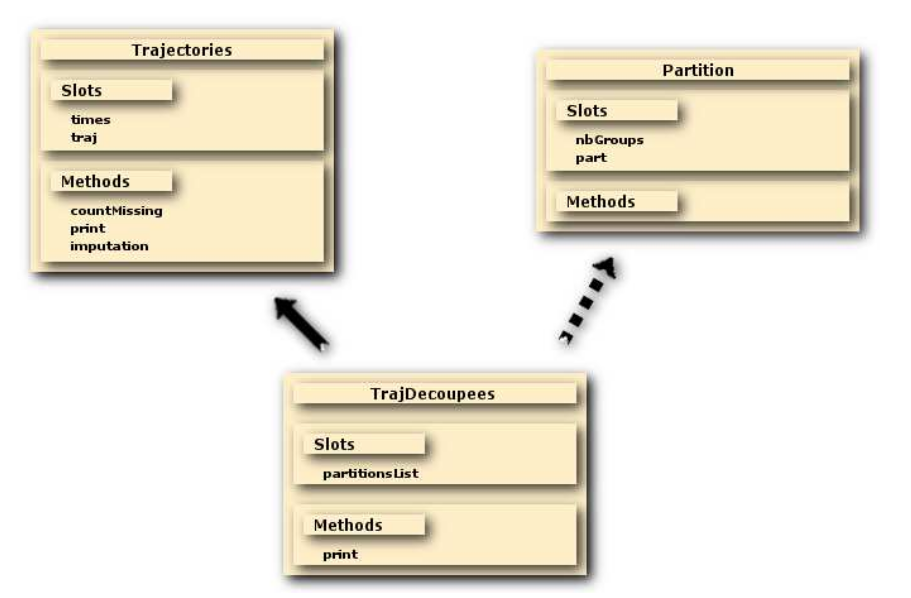
\includegraphics[width=5in]{./screenshot02.png}
\caption{}
\label{}
\end{figure} 

\subsection{运用于R}
所以,R怎么样,你是不是正好也问这个问题。这是一个对象语言的其他特性,我们会做一个相对全面的分析(彻底地根据我们的问题的简化的版本(?????))并且这里仍然没有涉及到R。理论上,我们甚至可以悬着其他语言来编程,但是此时此刻这不是我们需要讨论的主题。
运用R,在2.1.2中定义的方法变成了这样的:
\begin{description}
  \item[构建方法:]主要的构建方法,承担这给类起名字的作用
  \item[检查:]这会依赖与对象
  \item[对属性的操作:]对于每一个属性,需要给定获取它的值的方法以及修改它的值的方法。
  \item[其他:]其他的方法依赖与对象的特征,除了发布(posting?)方法。对于发布,当输入一个名字的时候,show允许在控制台中发布对象的基本的信息。(???????)。print函数会给更加复杂的发布。plot是图像的发布函数。
\end{description}

\scalebox{4}{\HandRight}为了使用R语言的特性来完成这个工作,大部分的面向对象的语言强制程序员在同一个地方组织所有的东西和一个对象向关联。我们称之为封装。R没有这种性质:你可以删除一个对象,然后删除另外一个,然后删除第一个对象的方法,然后删除第三个对象,如此等等。这是很坏的事情!如果使用以下的一个简单的规则那么就是可以避免上面的麻烦:就是一个对象一个文件。所有包含在一个对象中的东西必须储存在一个文件中,一个文件应当包含只和一个对象关联的对象。所以对于其他的对象,仅仅是发来其他的文件。


\part{面向对象编程的基础}
\section{类的定义}
\scalebox{4}{\HandRight}在大多数的面向对象的语言中,对象的定义包含槽和方法。在R中,定义仅仅包括槽。方法会在后来被指定。这是很遗憾的,这削弱了封装的功效,但是情况就是这样。明白内情的用户(比如说是你)可以通过强制地在统一个文件中定义槽和方法并不其对于每一个对象使用一个文件夹来“人为”地改变这些。这会更加清晰。
更加高级的关于封装的艺术可以参看章节B.6.
\subsection{定义槽}
第一步是定义对象自身的槽。这可以通过使用setClass完成。setClass包含了两个参数(以及一些我们以后会看到的其他成分)。
\begin{description}
  \item[Class:]表示的是我们要定义的类的名字
  \item[representation:]是对象的属性列表
\end{description}
如我们在介绍部分的例子中看到的,面向对象编程实现了类型的控制。这就意味着当必须是整数的地方是不允许储存字符串的。所以我们定义的时候必须要声明其类型。
\begin{knitrout}
\definecolor{shadecolor}{rgb}{0.969, 0.969, 0.969}\color{fgcolor}\begin{kframe}
\begin{alltt}
\hlfunctioncall{setClass}(Class = \hlstring{"Trajectories"}, representation = \hlfunctioncall{representation}(times = \hlstring{"numeric"}, 
    traj = \hlstring{"matrix"}))
\end{alltt}
\end{kframe}
\end{knitrout}


\scalebox{4}{\HandRight}不幸的是,这是通过使用列表来定义类型的(或者说定义地很不好)。我们别无选择,当我们使用列表的时候是坏的且不幸的。(?????)

\subsection{默认的构造器}
当一个类存在的时候,我们可以使用构造其new来构造这个类的一个对象。
\begin{knitrout}
\definecolor{shadecolor}{rgb}{0.969, 0.969, 0.969}\color{fgcolor}\begin{kframe}
\begin{alltt}
\hlfunctioncall{new}(Class = \hlstring{"Trajectories"})
\end{alltt}
\begin{verbatim}
## An object of class "Trajectories"
## Slot "times":
## numeric(0)
## 
## Slot "traj":
## <0 x 0 matrix>
\end{verbatim}
\end{kframe}
\end{knitrout}

正如你所注意到的那样,这个结果是很不容易看懂的,所以定义一个方法来提升这种情况是很重要的。我们在在章节5.2中处理这件事情。
\begin{knitrout}
\definecolor{shadecolor}{rgb}{0.969, 0.969, 0.969}\color{fgcolor}\begin{kframe}
\begin{alltt}
\hlfunctioncall{new}(Class = \hlstring{"Trajectories"}, times = \hlfunctioncall{c}(1, 3, 4))
\end{alltt}
\begin{verbatim}
## An object of class "Trajectories"
## Slot "times":
## [1] 1 3 4
## 
## Slot "traj":
## <0 x 0 matrix>
\end{verbatim}
\begin{alltt}
\hlfunctioncall{new}(Class = \hlstring{"Trajectories"}, times = \hlfunctioncall{c}(1, 3, 4), traj = \hlfunctioncall{matrix}(1:4, 
    ncol = 2))
\end{alltt}
\begin{verbatim}
## An object of class "Trajectories"
## Slot "times":
## [1] 1 3 4
## 
## Slot "traj":
##      [,1] [,2]
## [1,]    1    3
## [2,]    2    4
\end{verbatim}
\end{kframe}
\end{knitrout}

一个对象可以想R中其他值一样存储为一个变量。为了战士我们的陈述,我们打算构建一个小例子。三个医院加入了这项研究。这三个医院是Pitie Salpetriere(我们到现在还没有收到该医院的数据文件,为他们感到羞耻)Cochin和Saint-Anne:
\begin{knitrout}
\definecolor{shadecolor}{rgb}{0.969, 0.969, 0.969}\color{fgcolor}\begin{kframe}
\begin{alltt}
trajPitie <- \hlfunctioncall{new}(Class = \hlstring{"Trajectories"})
trajCochin <- \hlfunctioncall{new}(Class = \hlstring{"Trajectories"}, times = \hlfunctioncall{c}(1, 
    3, 4, 5), traj = \hlfunctioncall{rbind}(\hlfunctioncall{c}(15, 15.1, 15.2, 15.2), 
    \hlfunctioncall{c}(16, 15.9, 16, 16.4), \hlfunctioncall{c}(15.2, NA, 15.3, 15.3), 
    \hlfunctioncall{c}(15.7, 15.6, 15.8, 16)))
trajStAnne <- \hlfunctioncall{new}(Class = \hlstring{"Trajectories"}, times = \hlfunctioncall{c}(1:10, 
    (6:16) * 2), traj = \hlfunctioncall{rbind}(\hlfunctioncall{matrix}(\hlfunctioncall{seq}(16, 19, length = 21), 
    ncol = 21, nrow = 50, byrow = TRUE), \hlfunctioncall{matrix}(\hlfunctioncall{seq}(15.8, 
    18, length = 21), ncol = 21, nrow = 30, byrow = TRUE)) + 
    \hlfunctioncall{rnorm}(21 * 80, 0, 0.2))
\end{alltt}
\end{kframe}
\end{knitrout}


\subsection{获得槽的值}
\scalebox{4}{\HandRight}本节所有的内容都是很危险的\scalebox{4}{\HandLeft}
获取槽的值使用的是@符号
\begin{knitrout}
\definecolor{shadecolor}{rgb}{0.969, 0.969, 0.969}\color{fgcolor}\begin{kframe}
\begin{alltt}
trajCochin@times
\end{alltt}
\begin{verbatim}
## [1] 1 3 4 5
\end{verbatim}
\begin{alltt}
trajCochin@times <- \hlfunctioncall{c}(1, 2, 4, 5)
trajCochin
\end{alltt}
\begin{verbatim}
## An object of class "Trajectories"
## Slot "times":
## [1] 1 2 4 5
## 
## Slot "traj":
##      [,1] [,2] [,3] [,4]
## [1,] 15.0 15.1 15.2 15.2
## [2,] 16.0 15.9 16.0 16.4
## [3,] 15.2   NA 15.3 15.3
## [4,] 15.7 15.6 15.8 16.0
\end{verbatim}
\end{kframe}
\end{knitrout}

正如我们稍后要看到了,我们应当避免使用@符号。事实上,它是不会调用检查方法的。我们当前使用的方法(会进行值域的发布或者更坏情况下,会把值分配给值域)在大多数情况下应该禁止使用。
在这个例子中,最终的用户应当从来不许要使用到它。

\scalebox{4}{\HandRight}它可能会使用到函数attr和函数attributes,但是这可能更加糟糕:如果你仅仅是作出了一个简单的输入错误,那么这就引起很坏很坏很坏的结果!

\subsection{默认值}
可以使用给定初始值来声明一个对象。对于每一次构建,如果用户没有特别声明槽的值的话,他们也还是有值的。因此,在定义一个对象的时候必须加上参数prototype:
\begin{knitrout}
\definecolor{shadecolor}{rgb}{0.969, 0.969, 0.969}\color{fgcolor}\begin{kframe}
\begin{alltt}
\hlfunctioncall{setClass}(Class = \hlstring{"TrajectoriesBis"}, representation = \hlfunctioncall{representation}(time = \hlstring{"numeric"}, 
    traj = \hlstring{"matrix"}), prototype = \hlfunctioncall{prototype}(time = 1, 
    traj = \hlfunctioncall{matrix}(0)))
\end{alltt}
\end{kframe}
\end{knitrout}

\scalebox{4}{\HandRight}在以前,定义默认的初始值是很又必要的一件事情,但一个变量没有被初始化的时候,一个危险就被写入了内存系统(设置是一件极其可怕的事情)。在现在,R和其谈大部分编程语言而言,这样的情况不再会发上了。如果没有声明一个值域,R会被对象赋一个适当的空值。

从哲学的角度来说,但一个对象被建立的时候,一种情况是知道它的值,在这种情况下是可以改变它的,或者不知道它的值,在这种情况下我们是没有理由给其赋值的。使用默认的初始值不是对古老往事的回忆而是处于实用的目的。这些值无论如何不应当被使用(It should not be used anymore)。

此外[[[dans le feu de l’action]]],这还会发生在某人忘记个给对象赋真实值的时候。如果存在默认值,那么默认值就会被使用。如果没有初始值,这就可能引起错误。在这特殊的情况下,这可能是很好,错误会引起我们的注意是我们发现我们忘记赋值了并且予以修改。因此,应该避免个默认值赋予值而是应该使其为空。

\subsection{删除对象}






\end{document}
